\section{Project Management Essentials}

Managing engineering projects is not an easy task. There is potential for requirement scope creep and given the lead-times in a products design, there is a lot of staff churn and unforeseen issues that might arise. In this section, we will be introducing you to a set of essential project management tools and methods that are used in industry. These are:

\begin{itemize}
    \item Action Tracking;
    \item \acf{BOM};
    \item \acf{PERT};
    \item Risk Mitigation; and,
    \item Cost/Resource Modelling
\end{itemize}


\subsection{Action Tracking}

Action tracking is the activity of assigning and monitoring of actions amongst team members within a project. Typically performed at meetings, actions are recorded and then assigned an owner whose responsible for getting the action completed. This does not necessarily mean doing the action themselves and subsequent delegation and/or teamwork may be required to support the owner in completing the action. Many companies employ action tracking to ensure project progression and maintaining balanced workloads amongst their employees.

Action trackers can come in many forms but a typical set-up is to use a spreadsheet as shown in \cref{tab:action-tracker}.

\begin{table*}[h]
    \centering
    \resizebox{\textwidth}{!}{
    \begin{tabular}{r l l r r r r r}
        \toprule
            \# & Action & Owner & Date Created & Date Completed & Hours Allocated & Hours Accrued & Status \\
        \midrule
            1 & An example action & EG & 01/01/1980 & 10/01/1980 & 2.00 & 3.00 & Completed \\
            2 & Another example & EG & 03/01/1980 & 20/01/1980 & 3.00 & 3.00 & Incomplete \\
        \bottomrule
    \end{tabular}
    }
    \caption{Example Action Tracker}
    \label{tab:action-tracker}
\end{table*}

\subsection{Bill of Materials}

A \acf{BOM} is a list of the raw materials, sub-assemblies, intermediate assemblies, sub-components, parts and the quantities of each needed to manufacture an end product. This often comes in the form of a spreadsheet but it is more and more common to have the \ac{BOM} generated by the \acf{CAD}/\acf{PLM} systems used by the company. The key benefit is that that \ac{BOM} will automatically update to include any design changes that are made by the engineers.


\subsection{Project Evaluation and Review Techniques (PERT)} 

\acf{PERT} are methods of analysing the tasks involved in completing a given project, especially the time needed to complete each task, to identify the minimum time needed to complete the project\cite{vanhoucke2012}. 
It can be considered to be a sub-section of graph theory where the aim is to identify the critical paths between tasks.

It incorporates uncertainty by making it possible to schedule a project while not knowing precisely the details and durations of all the activities. It is more of an event-oriented technique rather than start/completion -oriented, and is used more in projects where time is the major factor rather than cost. It has been applied to many large-scale, one-time, complex, non-routine infrastructure and Research \& Development projects.

\ac{PERT} involves the generation of a graph where the vertices refer to tasks and the edges represent dependencies between the tasks. In contrast to \acf{CPM}, where the edges would be weighted by a single metric, \ac{PERT} applies three metrics for the time it will take for an activity to complete. \ac{PERT} defines four types of time relating to an activity.

\begin{table}
  \small
  \begin{tabular}{r p{0.7\textwidth}}
    Optimistic & The minimum possible time required to accomplish an activity ($o$) or a path ($O$), assuming everything proceeds better than is normally expected. \\
    Pessimistic & The maximum possible time required to accomplish an activity ($p$) or a path ($P$), assuming everything goes wrong (but excluding major catastrophes). \\
    Most Likely Time & The best estimate of the time required to accomplish an activity ($m$) or a path ($M$), assuming everything proceeds as normal. \\
    Expected Time & The best estimate of the time required to accomplish an activity ($e$) or a path ($E$), which is derived from the previous time estimates using \cref{equ-time}.
  \end{tabular}
\end{table}

\begin{equation}
  e = \frac{o+4m+p}{6}
  \label{equ-time}
\end{equation}

One can also calculate the standard deviation for the expected time based on $o$ and $p$.

\begin{equation}
  \sigma_e = \frac{p-o}{6}
\end{equation}

With these metrics and the activity graph, we are then able to determine:

\begin{table}
  \small
  \begin{tabular}{r p{0.7\textwidth}}
    Float (Slack) & This a measure of the excess time and resources available to complete a task. It is the amount of time that a project task can be delayed without causing a delay in any subsequent tasks (free float) or the whole project (total float). Positive float would indicate ahead of schedule; negative float would indicate behind schedule; and zero float would indicate on schedule. \\
    Critical Path & The longest possible continuous pathway taken from the initial event to the terminal event. It determines the total calendar time required for the project; and, therefore, any time delays along the critical path will delay the reaching of the terminal event by at least the same amount. \\
    Critical Activity & An activity that has total float equal to zero. An activity with zero float is not necessarily on the critical path since its path may not be the longest. \\
    Lead time & The time by which a predecessor event must be completed in order to allow sufficient time for the activities that must elapse before a specific \ac{PERT} event reaches completion. \\
    Lag time & The earliest time by which a successor event can follow a specific \ac{PERT} event. \\
    Fast Tracking & Performing critical activities in parallel. \\
    Crashing Critical Path & Shortening duration of critical activities. \\
  \end{tabular}
\end{table}


\cref{tbl-project}\marginnote{Example} contains seven tasks that represent the work that needs to be performed for a project. Some tasks have dependencies on others whilst some tasks can be performed concurrently. The time estimates for the tasks have been provided for each of the tasks. In your case, these tasks would represent the manufacture, handling and assembly times for your Design \& Make.

\begin{table}[h!]
  \centering
  \begin{tabular}{l l r r r r}
  \toprule
    Activity & Predecessor & \multicolumn{4}{c}{Time Estimates} \\
    & & $o$ & $m$ & $p$ & $e$ \\
  \midrule
    A & -- & 2 & 4 & 6 & 4.00 \\
    B & -- & 3 & 5 & 9 & 5.33 \\
    C & A & 4 & 5 & 7 & 5.17 \\
    D & A & 4 & 6 & 10 & 6.33 \\
    E & B, C & 4 & 5 & 7 & 5.17 \\
    F & D & 3 & 4 & 8 & 4.50 \\
    G & E & 3 & 5 & 8 & 5.17 \\
  \bottomrule
  \end{tabular}
  \caption{Example project}\label{tbl-project}
\end{table}

From this information, we can generate a graph showing how the tasks are connected with one another (Figure~\ref{fig-pert-graph}). Each vertex in the graph contains:

\begin{itemize}
  \item Task name
  \item Expected Time ($e$)
  \item Early start time (ES)
  \item Early finish time (EF)
  \item Late start time (LS)
  \item Late finish time (LF)
  \item Float
\end{itemize}

To calculate these values, the process is as follows:

\begin{description}
  \item[Step 1] Calculate the Early Start ($ES$) and Early Finish ($EF$) times for each vertex.
  \item[Step 2] Calculate the Late Start ($LS$) and Late Finish ($LF$) times for each vertex.
  \item[Step 3] Calculate the float for each vertex and identify the critical path.
\end{description}

The results are this process is shown in Figure~\ref{fig-pert-graph}

Step 1\marginnote{Step One} is to calculate the Early Start ($ES$) and Early Finish ($EF$) times for each vertex. $ES$ is defined as the maximum $EF$ of all predecessor activities, unless the activity in question is the first activity, for which $ES=0$. EF is ES plus the expected task duration ($e$).

\begin{equation}
  EF = ES + e
\end{equation}

If\marginnote{Step Two} everything runs smoothly, the project should take 19.51 work days to complete. With this information, we can work backwards to determine the Late Start ($LS$) and Late Finish ($LF$) times for each task. $LF$ is defined as the minimum $LS$ of all successor activities, unless the activity is the last activity, for which the $LF=EF$. The $LS$ is the $LF$ minus the task duration.

\begin{figure*}[t!]
    \centering
    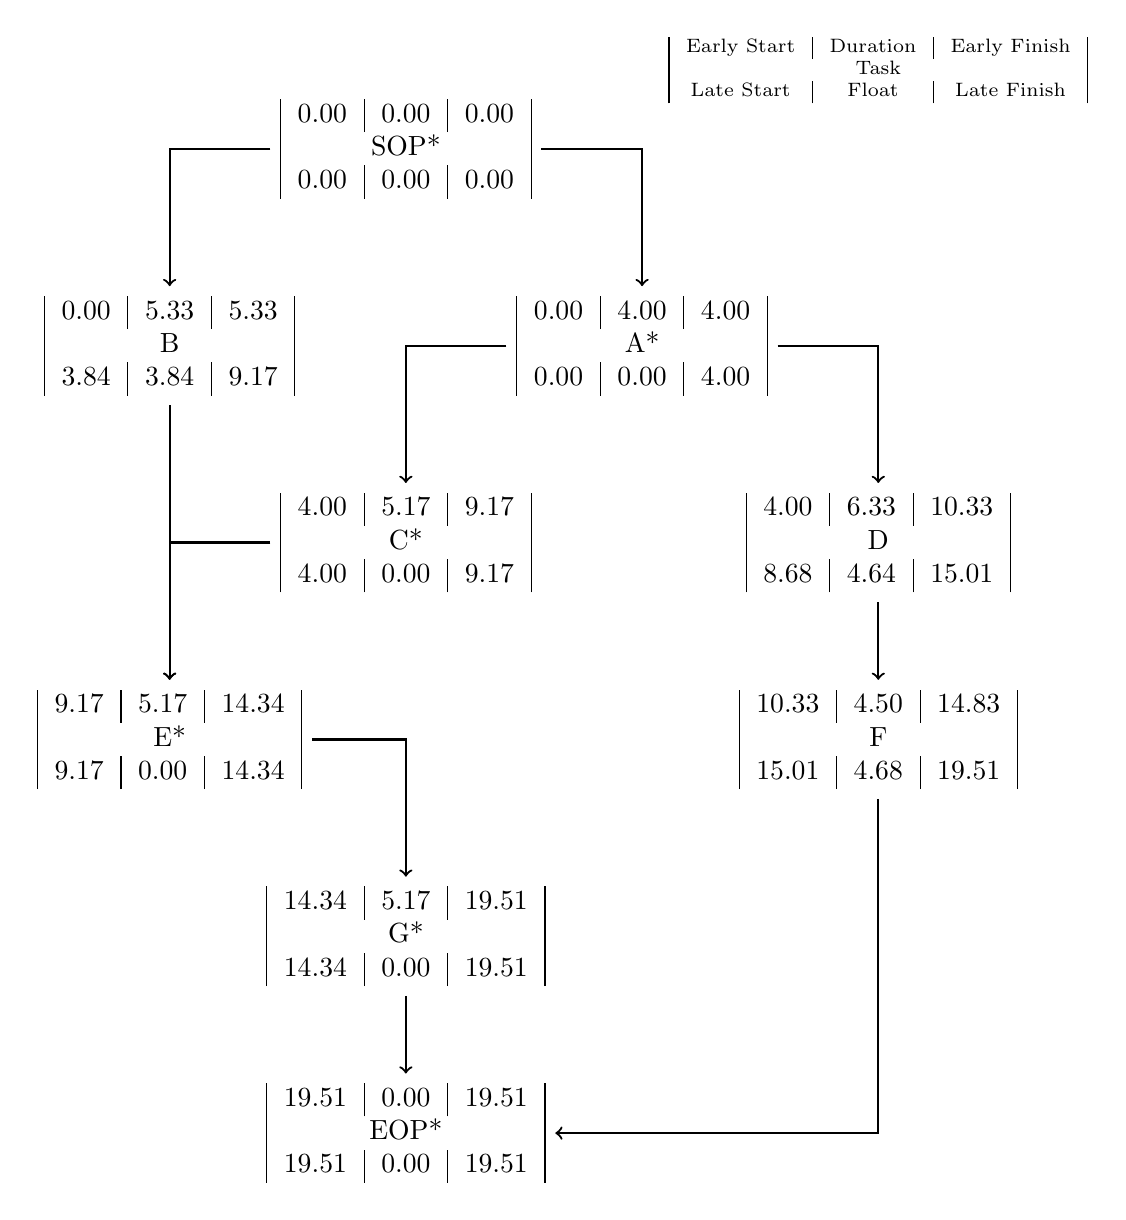
\begin{tikzpicture}

    \node[] (SOP) at (0,0) {
      \begin{tabular}{|c|c|c|}
        \midrule
          0.00 & 0.00 & 0.00 \\
        \midrule
          \multicolumn{3}{|c|}{SOP*} \\
        \midrule
          0.00 & 0.00 & 0.00 \\
        \midrule
      \end{tabular}
    };

    \node[] (A) at (3,-2.5) {
      \begin{tabular}{|c|c|c|}
        \midrule
          0.00 & 4.00 & 4.00 \\
        \midrule
          \multicolumn{3}{|c|}{A*} \\
        \midrule
          0.00 & 0.00 & 4.00 \\
        \midrule
      \end{tabular}
    };

    \node[] (B) at (-3,-2.5) {
      \begin{tabular}{|c|c|c|}
        \midrule
          0.00 & 5.33 & 5.33 \\
        \midrule
          \multicolumn{3}{|c|}{B} \\
        \midrule
          3.84 & 3.84 & 9.17 \\
        \midrule
      \end{tabular}
    };

    \node[] (D) at (6,-5) {
      \begin{tabular}{|c|c|c|}
        \midrule
          4.00 & 6.33 & 10.33 \\
        \midrule
          \multicolumn{3}{|c|}{D} \\
        \midrule
          8.68 & 4.64 & 15.01 \\
        \midrule
      \end{tabular}
    };

    \node[] (C) at (0,-5) {
      \begin{tabular}{|c|c|c|}
        \midrule
          4.00 & 5.17 & 9.17 \\
        \midrule
          \multicolumn{3}{|c|}{C*} \\
        \midrule
          4.00 & 0.00 & 9.17 \\
        \midrule
      \end{tabular}
    };

    \node[] (F) at (6,-7.5) {
      \begin{tabular}{|c|c|c|}
        \midrule
          10.33 & 4.50 & 14.83 \\
        \midrule
          \multicolumn{3}{|c|}{F} \\
        \midrule
          15.01 & 4.68 & 19.51 \\
        \midrule
      \end{tabular}
    };

    \node[] (E) at (-3,-7.5) {
      \begin{tabular}{|c|c|c|}
        \midrule
          9.17 & 5.17 & 14.34 \\
        \midrule
          \multicolumn{3}{|c|}{E*} \\
        \midrule
          9.17 & 0.00 & 14.34 \\
        \midrule
      \end{tabular}
    };

    \node[] (G) at (0,-10) {
      \begin{tabular}{|c|c|c|}
        \midrule
          14.34 & 5.17 & 19.51 \\
        \midrule
          \multicolumn{3}{|c|}{G*} \\
        \midrule
          14.34 & 0.00 & 19.51 \\
        \midrule
      \end{tabular}
    };

    \node[] (EOP) at (0,-12.5) {
      \begin{tabular}{|c|c|c|}
        \midrule
          19.51 & 0.00 & 19.51 \\
        \midrule
          \multicolumn{3}{|c|}{EOP*} \\
        \midrule
          19.51 & 0.00 & 19.51 \\
        \midrule
      \end{tabular}
    };

    \node[] (Index) at (6,1) {
      \scriptsize
      \begin{tabular}{|c|c|c|}
        \midrule
          Early Start & Duration & Early Finish \\
        \midrule
          \multicolumn{3}{|c|}{Task} \\
        \midrule
          Late Start & Float & Late Finish \\
        \midrule
      \end{tabular}
    };

    \draw[thick, ->] (SOP) -| (A);
    \draw[thick, ->] (SOP) -| (B);
    \draw[thick, ->] (A) -| (C);
    \draw[thick, ->] (A) -| (D);
    \draw[thick, ->] (B) -- (E);
    \draw[thick, ->] (C) -| (E);
    \draw[thick, ->] (D) -- (F);
    \draw[thick, ->] (E) -| (G);
    \draw[thick, ->] (F) |- (EOP);
    \draw[thick, ->] (G) -- (EOP);

    \end{tikzpicture}
    \vspace{1em}
    \caption{Project task graph}\label{fig-pert-graph}
\end{figure*}


\begin{equation}
  LS = LF - e
\end{equation}

Having\marginnote{Step Three} calculated $LS$ and $LF$ for each task, we can calculate the float for each activity. Float is equal to $LF - EF$ or $LS - ES$ as these are equivalent. This enables us to identify the critical path activities, which are indicated by the task having zero float.

%\marginlabel{Gantt Chart}

This\marginnote{Further Analysis} is as far as we will go with \ac{PERT} analysis for the Design \& Make exercise however, there is much more analysis that can be performed using this graph to provide organisations more information on the potential risk within the project. One example is the ability to automate the generation of these values so that you can perform a Monte-Carlo simulation based on the time distributions (known as \ac{PERT}-beta distributions). This analysis can provide insights in the potential variance in the critical path and the likelihood of the path changing depending on the task times\cite{davis2008}.

More advanced \ac{PERT} analysis also enables the inclusion of resource constraints, which limit the number of concurrent tasks. This could be due to a limitation in the availability of labour, machines and/or costed time.

A Python Notebook of the \ac{PERT} analysis procedure is available at: \\ \url{https://tinyurl.com/y72kjxfo}


\subsection{Risk Mitigation} 

All engineering projects carry risks and it is important to capture and monitor the potential risks as a project progresses. It is the duty of engineers to communicate risks clearly and effectively, and to propose solutions that will aid in mitigating risks to a project. In fact, we have already started to look at risks by using PERT to analyse and map out the plan of tasks for the project.

One\marginnote{Risk Register} method of capturing and monitoring risks within an engineering project is through the development of a risk register (\cref{tbl-risk}).

\begin{table}[h!]
  \centering
  \caption{Example Risk Register}
  \label{tbl-risk}
  \begin{tabular}{l l l l l l}
    \toprule
      No. & Risk & Impact & Chance & Owner & Mitigation \\
    \midrule
      1 \\
      2 \\
      3 \\
      \ldots \\
    \bottomrule
  \end{tabular}
\end{table}

An\marginnote{Example Risk} example in the Design \& Make project would be that a manufacturing machine (e.g\ Laser Cutter) for the manufacture of a gear is offline and requires maintenance. The impact of this is that a component will not be manufactured in time. The chance of this occurring is often attained through analysis of historical project data and analysis of the reliability of the machine. The owner may be the project manager but ideally risks should be equally shared amongst the team. So in this case, it may be best to give this risk to the engineer who designed and analysed the manufacturability of the product. We then have to come up with a strategy to mitigate the impact of this risk to the project. For this example, suggestions could be to have a alternative manufacturing strategy such as 3D printing or to purchase a gear from a supplier at an additional cost to the project.

Risks cover as many potential issues that the project could encounter. You should also be including issues where one of the team may be absent during the week that you intend to manufacture \& assemble the product.

This register will be very important during 2nd semester and during the presentation of your prototype, we would like you to reflect on the production of the product and whether you encountered any of these risks as well as any other issues that may have not been identified.

\subsection{Cost/Resource Modelling}

There are numerous sources that impact the cost and level of resource required for a project. In this exercise, we want to broaden your understanding of what cost means to a project and where it might come from.

During\marginnote{suppliers} your design work, you have been looking at supplier catalogues for potential sources of components. In this exercise, you will be solely focusing on the price of the components they offer but in a large organisation there are additional costs incurred such as contracts, stakeholder engagement, logistics and the resolving of issues if components are not to specification. 

For\marginnote{raw materials} each component you will be manufacturing in-house, there is a cost associated with the raw materials that you will be purchasing. As with the stock market, raw materials prices can change on a regular basis based on supply and demand at the time. Thus, large organisations often have to hedge and buy material in advance to have security that the material will be available to them but this also comes at an additional cost.

This\marginnote{machining} is the cost of manufacturing the components that you have designed. In this project, you have looked at the time to machine a single prototype component but in production projects there are additional costs such as those relating to the maintenance of the machines, cost of tooling (drill bits, dies, coolant) and energy/facility use.

In\marginnote{assembly} addition to machining, there is the cost of assembly, which you have been analysing during the design of your product. Again, there would be additional costs in the facilities required for this assembly line to function and the need to store components before and after assembly.

Then\marginnote{human resources} there is the human resource involved in the project and this is covers all the time spent designing, manufacturing and the cost of the personnel that need to be involved, which features pay scales, national insurance contributions, holiday entitlements and pensions to name a few. All these are factored into an engineers' hourly rate when being costed to projects.

In\marginnote{currency exchange rates} large organisations, the currency exchange rates can play a huge factor in to revenue and cost modelling of projects. This is where companies have order books looking ahead 20 years and predictions have to be made on the price the quote and the future cost. One example of the consequence of exchanges rates is Rolls-Royce having to write-down \textsterling2bn after the brexit vote due to the dip in the pound.\cite{tovey2016}

The list could continue and include:

\begin{itemize}
  \item Waste handling
  \item End-of-life recycling
  \item Logistics
  \item Offices
  \item Administrative services
  \item Maintenance \& service agreements
\end{itemize}
